\documentclass{letter}

\usepackage[key]{fbtest}
\usepackage{amsmath}
\usepackage{graphicx}

\begin{document}

  \begin{problem}{}
    Our rocket's engine provides 30 m/s\textsuperscript{2} of acceleration
    for 4 seconds, after which the rocket is in freefall.

    \subproblem{}{
      Write the acceleration $a(t)$ as a piecewise function of time $t$
      (use $-$10 m/s\textsuperscript{2} for acceleration due to gravity),
      and sketch the graph on domain $0 \leq t \leq 20$.

      \solution{
        \[
          a(t) = \begin{cases}
            20 \qquad\text{when } 0 \leq t \leq 4 \\
            -10 \qquad\text{when } t > 4
          \end{cases}
        \]

        \begin{center}
          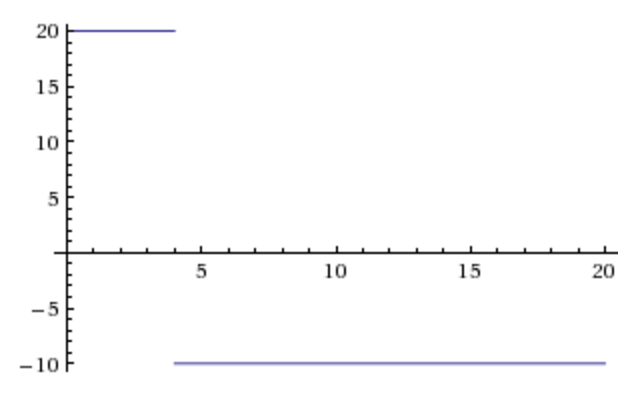
\includegraphics[width=0.5\textwidth]{graphic1.png}
        \end{center}
      }
    }

    \subproblem{}{
      Write the velocity $v(t)$ as a piecewise function of time $t$
      (make sure that it's continuous),
      and sketch the graph on domain $0 \leq t \leq 20$.
      When will the velocity be zero?

      \solution{
        \[
          v(t) = \begin{cases}
            20t \qquad\text{when } 0 \leq t \leq 4 \\
            -10t + 120 \qquad\text{when } t > 4
          \end{cases}
        \]

        \begin{center}
          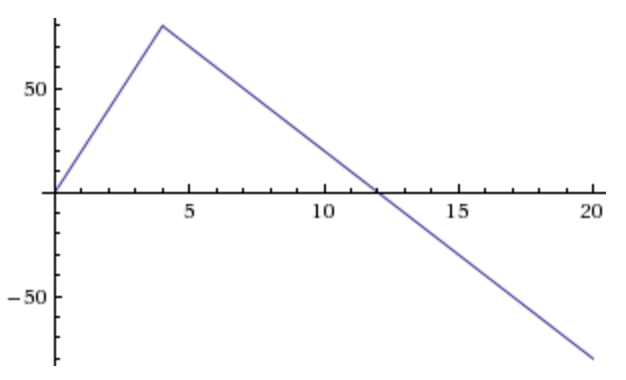
\includegraphics[width=0.5\textwidth]{graphic2.png}
        \end{center}

        The velocity is zero at $t = 12$.
      }
    }

    \subproblem{}{
      Write the height $h(t)$ as a piecewise function of time $t$.
      When is $h(t)$ at its maximum?

      \solution{
        \[
          h(t) = \begin{cases}
            10t^2 \qquad\text{when } 0 \leq t \leq 4 \\
            -5t^2 + 120t - 240 \qquad\text{when } t > 4
          \end{cases}
        \]

        The rocket reaches its max height at $t = 12$.
      }
    }

    \subproblem{}{
      What is the maximum height of our rocket?

      \solution{
        The maximum height is $h_\text{max} = h(12) = 480$.
      }
    }
  \end{problem}

  \begin{problem}{}
    Our rocket's engine provides 100 m/s\textsuperscript{2} of acceleration.
    We need our rocket to have a maximum height of 160,000 m (low-Earth
    orbit is approximately 160 km).
    We must decide how many seconds of fuel to give our rocket.
    How many seconds of fuel should we use in order for our rocket
    to have the desired maximum height?

    \solution{
      The number of seconds we burn the engine is an unknonwn, so we need
      to give it a name. Here we'll call it $A$.

      \[
        a(t) = \begin{cases}
          90 \qquad\text{when } 0 \leq t \leq A \\
          -10 \qquad\text{when } t > A
        \end{cases}
      \]

      We can write $v(t)$ using antiderivatives.

      \[
        v(t) = \begin{cases}
          90t \qquad\text{when } 0 \leq t \leq A \\
          -10t + C \qquad\text{when } t > A
        \end{cases}
      \]

      We're not doing writing $v(t)$, because we have to solve for the
      unknonw constant $C$.
      Make sure that $v(t)$ ends up being continuous by substituting
      $t = A$ into both expressions and equating:

      \begin{gather*}
        90A = -10A + C \\
        100A = C
      \end{gather*}

      We can now finish writing $v(t)$.

      \[
        v(t) = \begin{cases}
          90t \qquad\text{when } 0 \leq t \leq A \\
          -10t + 100A \qquad\text{when } t > A
        \end{cases}
      \]

      We do the same thing to find $h(t)$.

      \[
        h(t) = \begin{cases}
          45t^2 \qquad\text{when } 0 \leq t \leq A \\
          -5t^2 + 100At + C \qquad\text{when } t > A
        \end{cases}
      \]

      Solve for $C$ by setting $t = A$
      and equating the left and right branch.

      \begin{gather*}
        45A^2 = -5A^2 + 100A^2 + C \\
        -50T^2 = C
      \end{gather*}

      Finish writing $h(t)$.

      \[
        h(t) = \begin{cases}
          45t^2 \qquad\text{when } 0 \leq t \leq A \\
          -5t^2 + 100At -50A^2 \qquad\text{when } t > A
        \end{cases}
      \]

      $h(t)$ has its maximum when $v(t) = 0$.
      We need to find when $v(t) = 0$ (in terms of $A$).
      Since this will certainly be after the engines cut off,
      we use the $t > A$ branch of $v(t)$.

      \begin{gather*}
        0 = -10t + 100A \\
        t = 10A
      \end{gather*}

      So $h(t)$ has its maximum when $t = 10A$.

      \begin{gather*}
        h_\text{max} = h(10A) = -5(10A)^2 + 100A(10A) -50A^2
        h_\text{max} = 450A^2
      \end{gather*}

      So $h_\text{max} = 450A^2$. On the other hand, we know that we
      need $h_\text{max}$ to be 160,000, and we can use this to solve
      for $A$.

      \begin{gather*}
        160000 = 450A^2 \\
        355.\bar{5} = A^2 \\
        \sqrt{355.\bar{5}} = A \\
        18.856 \approx A
      \end{gather*}
    }
  \end{problem}

\end{document}
